%!TEX root = ../../main.tex
While we considered using various features for the character recognition such as crossing, projection histograms and celled projections \cite{HWR:features1}\cite{HWR:features2}. From all the above the celled projections report the best results (7\% and 10\% better than crossings and projections respectively) \cite{HWR:features1}. At this point it is also worth mentioning that we scaled the character pictures relatively to their height before extracting the features.


\subsubsection{Projection histogram}
Projection histogram \cite{Chacko2015} is simply the histogram of the letter on $x$ or $y$ axis or both. In \cref{fig:method:features:hist_proj} we see an example of projection histogram on a character.

\begin{figure}[ht]
	\centering
	
\includegraphics[width=8em]{shared/img/hist_project.png}
	\caption{Projection histogram of number 5. Image taken form \cite{oliveraugereau}.}
	\label{fig:method:features:hist_proj}
\end{figure}




\subsubsection{Celled projection}
Celled projections are extracted as follows. First the area of the character is split into regions, vertically, horizontally or mixed. In \ref{fig:method:features:feature} we see an example of vertical projection. Then for each of the regions we acquire the projections of the pixels on the left border of the region. This way binary vectors are created which then we concatenate.

\begin{figure}[t!]
	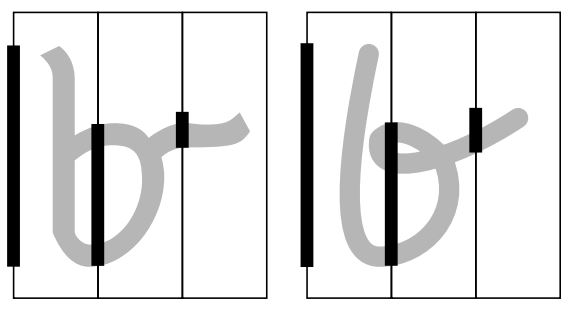
\includegraphics[width=8cm]{shared/img/projection_letter.jpg}
	\caption{In the above picture we see that even if the characters are differently written the projection feature will still extract consistent vectors.}
	\label{fig:method:features:feature}
\end{figure}

\subsubsection{Crossings}
Crossings is very similar to the projection histogram however instead of counting the foreground pixels (which is what histogram does) crossings count the alterations between foreground and background and store the number of alterations in an array. Once again, this can be performed in either the $x$ and $y$ axis.